\documentclass[a4paper,12pt,fleqn]{article}
\usepackage{fixltx2e}
\usepackage[utf8]{inputenc}
\usepackage{graphicx}
\usepackage{sidecap}
\usepackage{fancyhdr}
\usepackage{amssymb,amsmath}
\usepackage[swedish]{babel}
\usepackage[margin=1.5in]{geometry}
\usepackage{abstract}
\usepackage[parfill]{parskip}
\usepackage{tocloft}
\usepackage{adjustbox}
\usepackage{textcomp}
\usepackage[T1]{fontenc}
\usepackage{listings}
\usepackage{xcolor,colortbl}
\usepackage{hyperref}
\usepackage{mcode}
\usepackage{a4wide}
\usepackage{caption}

\begin{document}

\section{Inledning}

Vid kommunikation används ofta I-/Q-modulering för att överföra en signal inom ett givet frekvensutrymme. I och med överföringen kan tidsfördröjningar införas. I mottagaränden måste dessa tidsfördröjningar kompenseras för innan överföringen sedan kan I-/Q-demoduleras för att extrahera ljudinformationen 

\subsection{Syfte}

Syftet med denna laboration är att finna bärfrekvens för en given signal, filtrera bort oönskade delar av överföringen och sedan I-/Q-demodulera signalen för att extrahera relevant information. 

\subsection{Materiel och förutsättningar}

Filen signal-hanel742.wav är given med den kända samplingsfrekvensen 400 kHz. Givet är också att filen innehåller en smalbandig signal som är I-/Q-modulerad och har skickats genom filtret nedan. 

\begin{gather}
h(t) = \delta(t - \tau_1) + \delta(t - \tau_2)
\label{equ:filter}
\end{gather}

På förhand ges också att bärfrekvensen före relevant är en multipel av 19 kHz.

För att utföra laborationen används GNU Octave med vertygslådor för ljud samt signaler (octave-audio och octave-signal) installerat. 

% -------- Metod ------------
\newpage

\section{Metod}

Jag börjar med att läsa in filen i Octave och sedan fouriertransformera signalen för att få ut dess frekvensspektra: 

\begin{figure}[htp]
  \begin{center}
  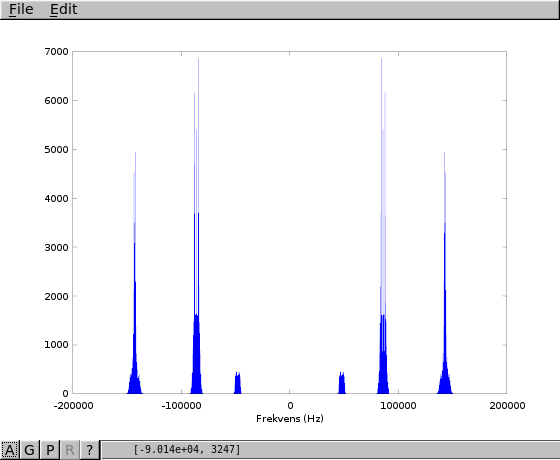
\includegraphics[keepaspectratio=true,width=\linewidth]{fft_orig_data.png}  %skala och filnamn. 
  \end{center}
  \caption{Dubbelsidigt amplitudspektrum för ursprunglig signal} %figurtext.
  \label{fig:fft_orig_data}
\end{figure}
\newpage

\subsection{Att finna bärfrekvens}

Jag vill nu filtrera ut signalelementen för de olika topparna ur totala signalen. För att skapa filter för tidsdiskreta signaler i Matlab eller Octave behöver man först normera frekvensgränserna. Topparnas normerade frekvens ges genom ekvation \ref{equ:normFreq}

\begin{gather}
normerad = \frac{frekvens \cdot 2}{samplingsfrekvens}
\label{equ:normFreq}
\end{gather}

Genom att utläsa frekvenserna ur topparna på graferna kan man se att topparna har bärfrekvenser i området kring frekvenserna i tabell \ref{table:carryfreq}. Topparna räknas från origo och utåt och filtrenas gränsfrekvens anges som normerad frekvens. 
~\\
\begin{center}
\begin{tabular}{c | c | c}
	\hline
	Topp & Ungefärlig bärfrekvens (Hz) & Filters gränsfrekvens \\ \hline
	1 & $4,959 \cdot 10^4$ & 0.2-0.4 \\ \hline
	2 & $8,313 \cdot 10^4$ & 0.5-0.65 \\ \hline
	3 & $1,412 \cdot 10^5$ & 0.7-0.8 \\ \hline
\end{tabular}
\captionof{table}{B{\"a}rfrekvenser} \label{table:carryfreq}
\end{center}
~\\
Filtrerar man sedan den givna signalen med hjälp av bandpassfilter med givna gränser ges utseende enligt figurer i appendix A. Enligt utseendet på graferna ser frekvenstopp 1 ut att innehålla någon form av information, medan den tredje toppen mest verkar innehålla vitt brus. 

Frekvenstopp 2 är mer svårbedömd - men en rimlig uppskattning är att den har ett alldeles för periodiskt utseende för att inehålla någon intressant information. 

Närmsta multipel av 19 kHz för den uppskattade bärfrekvensen för topp 1 är 57 kHz, vilket väljs till bärfrekvens för fortsatta experiment. 

\subsection{Filtrering}




% -------- Slutsatser ------------

\newpage
\section{Resultat och slutsats}
Jag har funnit att bla

% -------- Appendix ---------------

\newpage
\appendix
\pagestyle{empty}
\newgeometry{left=2cm,right=2cm,bottom=2cm,top=2cm}
\section{Filtrerade signaler}

\begin{figure}[htp]
  \begin{center}
  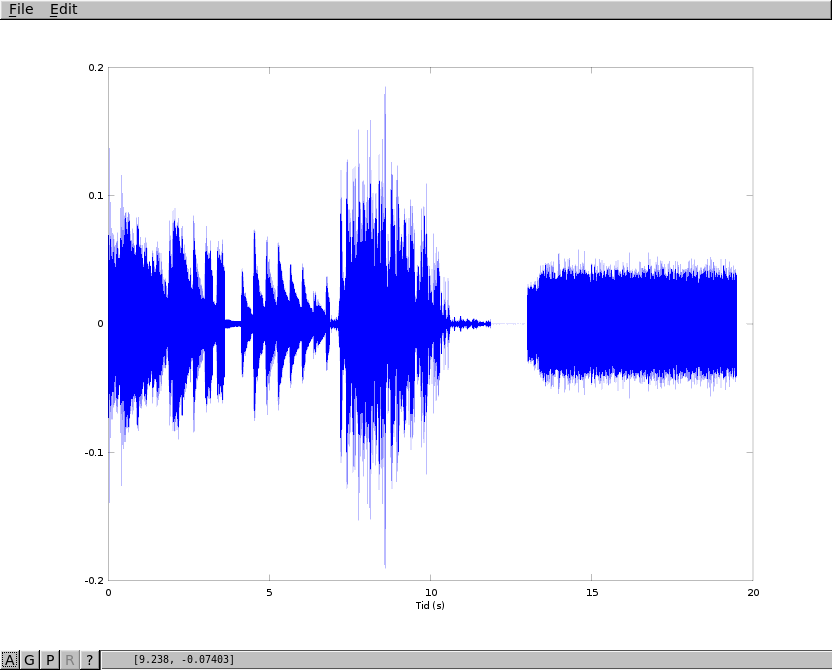
\includegraphics[keepaspectratio=true,width=\linewidth]{topp1_filter.png}  %skala och filnamn. 
  \end{center}
  \caption{Frekvenstopp 1 filtrerad} %figurtext.
  \label{fig:topp1_filter}
\end{figure}

\begin{figure}[htp]
  \begin{center}
  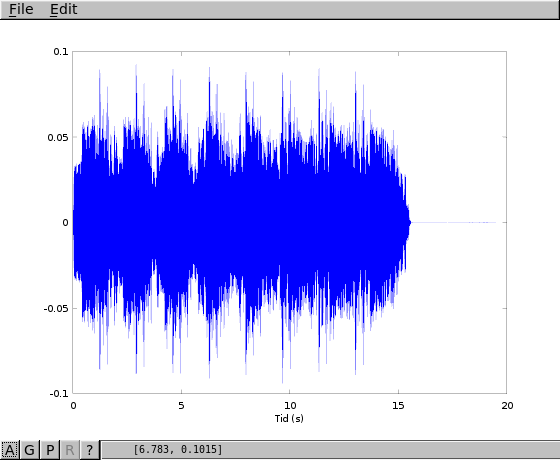
\includegraphics[keepaspectratio=true,width=\linewidth]{topp2_filter.png}  %skala och filnamn. 
  \end{center}
  \caption{Frekvenstopp 2 filtrerad} %figurtext.
  \label{fig:topp2_filter}
\end{figure}

\begin{figure}[htp]
  \begin{center}
  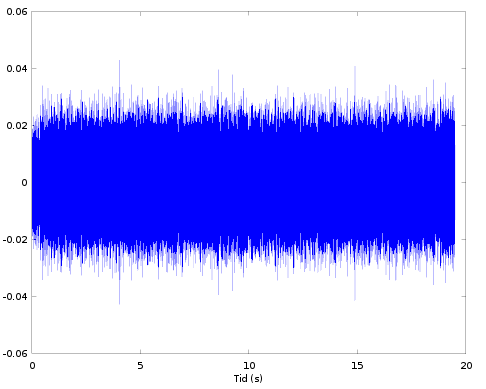
\includegraphics[keepaspectratio=true,width=\linewidth]{topp3_filter.png}  %skala och filnamn. 
  \end{center}
  \caption{Frekvenstopp 1 filtrerad} %figurtext.
  \label{fig:topp3_filter}
\end{figure}

\newpage
\section{Kod för GNU Octave}

\lstinputlisting{tsks10.m}

\end{document}